% answers.tex —— 1999 年·全国卷·文科 · 参考答案与详细解析片段
% 由 tools/generate_projects.py 依来源总账自 1999/1999_数学真题_全国文_试题.md + 1999/1999_数学真题_全国文_解析正文.md + 1999/1999_数学真题_全国文_答案要点.md 生成，勿手改（改源 MD 后重跑）


\begin{gktip}
固定源 PDF 只有一页题面，没有答案和解析页。以下各题均依据题面独立复算；第 1、10、22、23、24 题的图形在 LaTeX 工程中以 TikZ/PGFPlots 矢量源重绘。
\end{gktip}

\begin{answer}
\gksolhead{1}{}

\textbf{题目}：

如图，$I$ 是全集，$M$、$P$、$S$ 是 $I$ 的 3 个子集，则阴影部分所表示的集合是\mbox{（　　）}
\nopagebreak[4]
\begin{center}% 1999 年全国卷文科第 1 题：集合关系图
% 仅保留 TikZ 矢量源；阴影表示 (M \cap P) \cap \overline S。
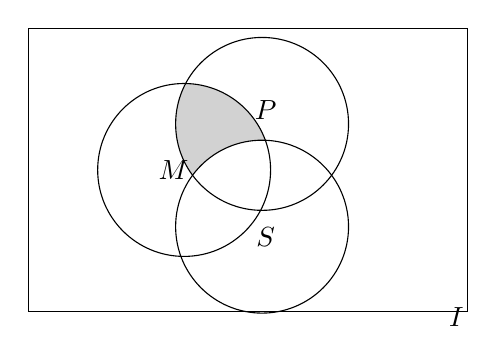
\begin{tikzpicture}[scale=0.9]
  \coordinate (M) at (2.2,2.0);
  \coordinate (P) at (3.3,2.65);
  \coordinate (S) at (3.3,1.2);

  \draw (0,0) rectangle (6.2,4.0);
  \begin{scope}
    \clip (M) circle (1.22);
    \clip (P) circle (1.22);
    \fill[gray!35] (0,0) rectangle (6.2,4.0);
  \end{scope}
  \fill[white] (S) circle (1.22);
  \draw (0,0) rectangle (6.2,4.0);
  \draw (M) circle (1.22);
  \draw (P) circle (1.22);
  \draw (S) circle (1.22);

  \node at (2.05,2.0) {$M$};
  \node at (3.35,2.85) {$P$};
  \node at (3.35,1.05) {$S$};
  \node[below right] at (5.8,0.2) {$I$};
\end{tikzpicture}
\end{center}
\nopagebreak[4]
（A）$(M\cap P)\cap S$　　（B）$(M\cap P)\cup S$

（C）$(M\cap P)\cap\overline S$　　（D）$(M\cap P)\cup\overline S$

\Needspace{4\baselineskip}
\textbf{解析}

\Needspace{5\baselineskip}
阴影区域同时属于 $M$、$P$，但不属于 $S$，所以所表示的集合为

\nopagebreak[4]
\[
(M\cap P)\cap\overline S.
\]

选 C。

\gkanswer{答案：C}

\end{answer}
\begin{answer}
\gksolhead{2}{}

\textbf{题目}：

已知映射 $f:A\to B$，其中，集合 $A=\{-3,-2,-1,1,2,3,4\}$，集合 $B$ 中的元素都是 $A$ 中元素在映射 $f$ 下的象，且对任意的 $a\in A$，在 $B$ 中和它对应的元素是 $|a|$，则集合 $B$ 中元素的个数是\mbox{（　　）}

（A）4　　（B）5　　（C）6　　（D）7

\Needspace{4\baselineskip}
\textbf{解析}

映射为 $a\mapsto|a|$。集合 $A$ 中元素的绝对值只有 $1,2,3,4$ 四种，所以 $B$ 有 4 个元素，选 A。

\gkanswer{答案：A}

\end{answer}
\begin{answer}
\gksolhead{3}{}

\textbf{题目}：

若函数 $y=f(x)$ 的反函数是 $y=g(x)$，$f(a)=b$，$ab\ne0$，则 $g(b)$ 等于\mbox{（　　）}

（A）$a$　　（B）$a^{-1}$　　（C）$b$　　（D）$b^{-1}$

\Needspace{4\baselineskip}
\textbf{解析}

\Needspace{5\baselineskip}
由反函数定义

\nopagebreak[4]
\[
f(a)=b\Longleftrightarrow g(b)=a.
\]

故选 A。

\gkanswer{答案：A}

\end{answer}
\begin{answer}
\gksolhead{4}{}

\textbf{题目}：

函数 $f(x)=M\sin(\omega x+\varphi)\ (\omega>0)$ 在区间 $[a,b]$ 上是增函数，且 $f(a)=-M$，$f(b)=M$，则函数 $g(x)=M\cos(\omega x+\varphi)$ 在 $[a,b]$ 上\mbox{（　　）}

（A）是增函数　　（B）是减函数

（C）可以取得最大值 $M$　　（D）可以取得最小值 $-M$

\Needspace{4\baselineskip}
\textbf{解析}

令 $t=\omega x+\varphi$。由于 $M\sin t$ 在给定区间递增，且端点值从 $-M$ 变为 $M$，相应的 $t$ 从 $-\dfrac\pi2+2k\pi$ 变化到 $\dfrac\pi2+2k\pi$，其中包含 $t=2k\pi$。所以 $M\cos t$ 可以取得最大值 $M$，选 C。

\gkanswer{答案：C}

\end{answer}
\begin{answer}
\gksolhead{5}{}

\textbf{题目}：

若 $f(x)\sin x$ 是周期为 $\pi$ 的奇函数，则 $f(x)$ 可以是\mbox{（　　）}

（A）$\sin x$　　（B）$\cos x$　　（C）$\sin2x$　　（D）$\cos2x$

\Needspace{4\baselineskip}
\textbf{解析}

\Needspace{5\baselineskip}
有

\nopagebreak[4]
\[
\sin x\cdot\sin x=\sin^2x
\]

\Needspace{5\baselineskip}
是偶函数，而

\nopagebreak[4]
\[
\cos x\cdot\sin x=\frac12\sin2x
\]

是周期为 $\pi$ 的奇函数。另两项分别不满足奇性或周期条件，故选 B。

\gkanswer{答案：B}

\end{answer}
\begin{answer}
\gksolhead{6}{}

\textbf{题目}：

曲线 $x^2+y^2+2\sqrt2x-2\sqrt2y=0$ 关于\mbox{（　　）}

（A）直线 $x=\sqrt2$ 轴对称　　（B）直线 $y=-x$ 轴对称

（C）点 $(-2,\sqrt2)$ 中心对称　　（D）点 $(-\sqrt2,0)$ 中心对称

\Needspace{4\baselineskip}
\textbf{解析}

\Needspace{5\baselineskip}
配方得

\nopagebreak[4]
\[
x^2+y^2+2\sqrt2x-2\sqrt2y=0
\Longleftrightarrow
(x+\sqrt2)^2+(y-\sqrt2)^2=4.
\]

这是圆心为 $(-\sqrt2,\sqrt2)$、半径为 $2$ 的圆。圆心在直线 $y=-x$ 上，因此该圆关于直线 $y=-x$ 轴对称，选 B。

\gkanswer{答案：B}

\end{answer}
\begin{answer}
\gksolhead{7}{}

\textbf{题目}：

将若干毫升水倒入底面半径为 $2\ \mathrm{cm}$ 的圆柱形器皿中，量得水面的高度为 $6\ \mathrm{cm}$，若将这些水倒入轴截面是正三角形的倒圆锥形器皿中，则水面的高度是\mbox{（　　）}

（A）$6\sqrt3\ \mathrm{cm}$　　（B）$6\ \mathrm{cm}$　　（C）$2\sqrt[3]{18}\ \mathrm{cm}$　　（D）$3\sqrt[3]{12}\ \mathrm{cm}$

\Needspace{4\baselineskip}
\textbf{解析}

\Needspace{5\baselineskip}
圆柱中水的体积为

\nopagebreak[4]
\[
V=\pi\cdot2^2\cdot6=24\pi\ \mathrm{cm^3}.
\]

\Needspace{5\baselineskip}
设倒圆锥水面的高度为 $h$，圆锥底面半径为 $r$。轴截面为正三角形，故 $h=\sqrt3r$；相似关系给出高度 $h$ 处的水面半径为 $h/\sqrt3$。于是

\nopagebreak[4]
\[
V=\frac13\pi\left(\frac h{\sqrt3}\right)^2h
=\frac{\pi h^3}{9}.
\]

令其等于 $24\pi$，得 $h=6\ \mathrm{cm}$，选 B。

\gkanswer{答案：B}

\end{answer}
\begin{answer}
\gksolhead{8}{}

\textbf{题目}：

若 $(2x+\sqrt3)^3=a_0+a_1x+a_2x^2+a_3x^3$，则 $(a_0+a_2)^2-(a_1+a_3)^2$ 的值为\mbox{（　　）}

（A）$-1$　　（B）1　　（C）0　　（D）2

\Needspace{4\baselineskip}
\textbf{解析}

\Needspace{5\baselineskip}
记 $P(x)=(2x+\sqrt3)^3$，令 $E=a_0+a_2$、$O=a_1+a_3$，则

\nopagebreak[4]
\[
E^2-O^2=P(1)P(-1)
=(2+\sqrt3)^3(\sqrt3-2)^3
=\bigl((2+\sqrt3)(\sqrt3-2)\bigr)^3=-1.
\]

选 A。

\gkanswer{答案：A}

\end{answer}
\begin{answer}
\gksolhead{9}{}

\textbf{题目}：

直线 $\sqrt3x+y-2\sqrt3=0$ 截圆 $x^2+y^2=4$ 得的劣弧所对的圆心角为\mbox{（　　）}

（A）$\dfrac\pi6$　　（B）$\dfrac\pi4$　　（C）$\dfrac\pi3$　　（D）$\dfrac\pi2$

\Needspace{4\baselineskip}
\textbf{解析}

\Needspace{5\baselineskip}
圆心到直线 $\sqrt3x+y-2\sqrt3=0$ 的距离为

\nopagebreak[4]
\[
d=\frac{2\sqrt3}{\sqrt{3+1}}=\sqrt3.
\]

\Needspace{5\baselineskip}
半弦长为 $\sqrt{2^2-d^2}=1$。若劣弧所对的圆心角为 $\theta$，则

\nopagebreak[4]
\[
1=2\sin\frac\theta2,
\qquad \theta=\frac\pi3.
\]

选 C。

\gkanswer{答案：C}

\end{answer}
\begin{answer}
\gksolhead{10}{}

\textbf{题目}：

如图，在多面体 $ABCDEF$ 中，已知面 $ABCD$ 是边长为 $3$ 的正方形，$EF\parallel AB$，$EF=\dfrac32$，$EF$ 与面 $ABCD$ 的距离为 $2$，则该多面体的体积为\mbox{（　　）}
\nopagebreak[4]
\begin{center}% 1999 年全国卷文科第 10 题：多面体 ABCDEF
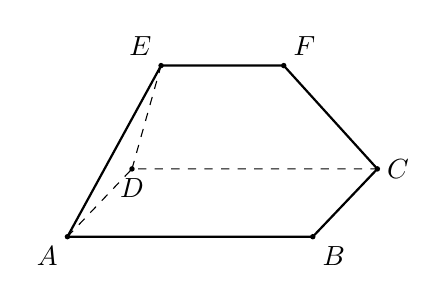
\begin{tikzpicture}[scale=0.82, >=stealth]
  \coordinate (A) at (0,0);
  \coordinate (B) at (3.8,0);
  \coordinate (C) at (4.8,1.05);
  \coordinate (D) at (1.0,1.05);
  \coordinate (E) at (1.45,2.65);
  \coordinate (F) at (3.35,2.65);

  \draw[thick] (A)--(B)--(C)--(F)--(E)--cycle;
  \draw[dashed] (A)--(D)--(C) (D)--(E);

  \fill (A) circle (1.2pt) node[below left] {$A$};
  \fill (B) circle (1.2pt) node[below right] {$B$};
  \fill (C) circle (1.2pt) node[right] {$C$};
  \fill (D) circle (1.2pt) node[below] {$D$};
  \fill (E) circle (1.2pt) node[above left] {$E$};
  \fill (F) circle (1.2pt) node[above right] {$F$};
\end{tikzpicture}
\end{center}
\nopagebreak[4]
（A）$\dfrac92$　　（B）5　　（C）6　　（D）$\dfrac{15}2$

\Needspace{4\baselineskip}
\textbf{解析}

\Needspace{5\baselineskip}
底面正方形面积为 $9$，顶边 $EF$ 到底面的距离为 $2$，且 $EF$ 长为 $\dfrac32$、平行于 $AB$。设高度参数为 $t\in[0,1]$，在高度 $2t$ 处，底面正方形按比例 $1-t$ 缩小，并沿 $AB$ 方向加上长度为 $\dfrac32t$ 的线段，因此截面面积为

\nopagebreak[4]
\[
A(t)=9(1-t)^2+\frac92t(1-t).
\]

\Needspace{5\baselineskip}
由切片积分

\nopagebreak[4]
\[
\begin{aligned}
V
&=2\int_0^1A(t)\,\mathrm dt\\
&=2\int_0^1\left(9(1-t)^2+\frac92t(1-t)\right)\mathrm dt\\
&=2\left(3+\frac34\right)
=\frac{15}{2}.
\end{aligned}
\]

选 D。

\gkanswer{答案：D}

\end{answer}
\begin{answer}
\gksolhead{11}{}

\textbf{题目}：

若 $\sin\alpha>\tan\alpha>\cot\alpha\ \left(-\dfrac\pi2<\alpha<\dfrac\pi2\right)$，则 $\alpha\in$\mbox{（　　）}

（A）$\left(-\dfrac\pi2,-\dfrac\pi4\right)$　　（B）$\left(-\dfrac\pi4,0\right)$

（C）$\left(0,\dfrac\pi4\right)$　　（D）$\left(\dfrac\pi4,\dfrac\pi2\right)$

\Needspace{4\baselineskip}
\textbf{解析}

\Needspace{5\baselineskip}
医生分配有 $3!=6$ 种，护士分组有

\nopagebreak[4]
\[
\binom62\binom42\binom22=90
\]

种，所以总数为 $6\times90=540$，选 D。

\gkanswer{答案：B}

\end{answer}
\begin{answer}
\gksolhead{12}{}

\textbf{题目}：

如果圆台的上底面半径为 $5$，下底面半径为 $R$，中截面把圆台分为上、下两个圆台，它们的侧面积的比为 $1:2$，那么 $R=$\mbox{（　　）}

（A）10　　（B）15　　（C）20　　（D）25

\Needspace{4\baselineskip}
\textbf{解析}

\Needspace{5\baselineskip}
中截面半径为 $\dfrac{R+5}{2}$。若圆台母线总长为 $l$，上、下两个小圆台的母线长均为 $l/2$，故侧面积之比为

\nopagebreak[4]
\[
\frac{5+\frac{R+5}{2}}{\frac{R+5}{2}+R}
=\frac{R+15}{3R+5}.
\]

令其等于 $\dfrac12$，得 $R=25$，选 D。

\gkanswer{答案：D}

\end{answer}
\begin{answer}
\gksolhead{13}{}

\textbf{题目}：

给出下列曲线方程：

① $4x+2y-1=0$；② $x^2+y^2=3$；③ $\dfrac{x^2}{2}+y^2=1$；④ $\dfrac{x^2}{2}-y^2=1$。

其中与直线 $y=-2x-3$ 有交点的所有曲线方程是\mbox{（　　）}

（A）①③　　（B）②④　　（C）①②③　　（D）②③④

\Needspace{4\baselineskip}
\textbf{解析}

\Needspace{5\baselineskip}
直接考察给出的直线

\nopagebreak[4]
\[
y=-2x-3.
\]

它与 $4x+2y-1=0$ 平行，所以①不符合。与圆 $x^2+y^2=3$ 相交，因为原点到该直线的距离 $3/\sqrt5<\sqrt3$。

\Needspace{5\baselineskip}
代入③得

\nopagebreak[4]
\[
\frac{x^2}{2}+(2x+3)^2=1
\Longleftrightarrow
(3x+4)^2=0,
\]

\Needspace{5\baselineskip}
故③相切。代入④得

\nopagebreak[4]
\[
\frac{x^2}{2}-(2x+3)^2=1
\Longleftrightarrow
7x^2+24x+20=0,
\]

判别式为 $16>0$，故④也有交点。因此选②③④，即选 D。

\gkanswer{答案：D}

\end{answer}
\begin{answer}
\gksolhead{14}{}

\textbf{题目}：

某电脑用户计划使用不超过 500 元的资金购买单价分别为 60 元、70 元的单片软件和盒装磁盘，根据需要，软件至少买 3 片，磁盘至少买 2 盒，则不同的选购方式共有\mbox{（　　）}

（A）5 种　　（B）6 种　　（C）7 种　　（D）8 种

\Needspace{4\baselineskip}
\textbf{解析}

\Needspace{5\baselineskip}
设软件买 $x$ 片、磁盘买 $y$ 盒，则

\nopagebreak[4]
\[
x\ge3,\qquad y\ge2,\qquad60x+70y\le500.
\]

当 $x=3,4,5,6$ 时，$y$ 的取值数分别为 $3,2,1,1$，总数为 $7$，选 C。

\gkanswer{答案：C}

\end{answer}
\begin{answer}
\gksolhead{15}{}

\textbf{题目}：

设椭圆 $\dfrac{x^2}{a^2}+\dfrac{y^2}{b^2}=1\ (a>b>0)$ 的右焦点为 $F_1$，右准线为 $l_1$，若过 $F_1$ 且垂直于 $x$ 轴的弦长等于点 $F_1$ 到 $l_1$ 的距离，则椭圆的离心率是\gkblank{}。

\Needspace{4\baselineskip}
\textbf{解析}

\Needspace{5\baselineskip}
设椭圆焦半距为 $c$，则 $c^2=a^2-b^2$。过右焦点且垂直于 $x$ 轴的弦长为

\nopagebreak[4]
\[
2b\sqrt{1-\frac{c^2}{a^2}}=\frac{2b^2}{a}.
\]

\Needspace{5\baselineskip}
右准线为 $x=\dfrac{a^2}{c}$，焦点到右准线的距离为

\nopagebreak[4]
\[
\frac{a^2}{c}-c=\frac{b^2}{c}.
\]

\Needspace{5\baselineskip}
由题意 $2b^2/a=b^2/c$，得 $c=a/2$，所以离心率

\nopagebreak[4]
\[
e=\frac ca=\frac12.
\]

\gkanswer{答案：$\dfrac12$}

\end{answer}
\begin{answer}
\gksolhead{16}{}

\textbf{题目}：

在一块并排 10 垄的田地中，选择 2 垄分别种植 $A$、$B$ 两种作物，每种作物种植一垄，为有利于作物生长，要求 $A$、$B$ 两种作物的间隔不小于 6 垄，则不同的选垄方法共有\gkblank{}种。（用数字作答）

\Needspace{4\baselineskip}
\textbf{解析}

把 10 垄编号为 $1,\ldots,10$，设所选编号为 $i<j$。两垄之间至少有 6 垄，故 $j-i\ge7$。编号差为 $7,8,9$ 时分别有 $3,2,1$ 对，合计 $6$ 种。

\gkanswer{答案：6}

\end{answer}
\begin{answer}
\gksolhead{17}{}

\textbf{题目}：

若正数 $a$、$b$ 满足 $ab=a+b+3$，则 $ab$ 的取值范围是\gkblank{}。

\Needspace{4\baselineskip}
\textbf{解析}

\Needspace{5\baselineskip}
由

\nopagebreak[4]
\[
(a-1)(b-1)=4.
\]

\Needspace{5\baselineskip}
因 $a,b>0$，两因子不可能同时为负，所以令 $t=a-1>0$，则 $b-1=4/t$。于是

\nopagebreak[4]
\[
ab=5+t+\frac4t\ge9,
\]

等号在 $t=2$ 时取得，故 $ab\in[9,+\infty)$。

\gkanswer{答案：$[9,+\infty)$}

\end{answer}
\begin{answer}
\gksolhead{18}{}

\textbf{题目}：

$\alpha$、$\beta$ 是两个不同的平面，$m$、$n$ 是平面 $\alpha$ 及 $\beta$ 之外的两条不同直线，给出四个论断：① $m\perp n$；② $\alpha\perp\beta$；③ $n\perp\beta$；④ $m\perp\alpha$。以其中三个论断作为条件，余下一个论断作为结论，写出你认为正确的一个命题：\gkblank{}。

\Needspace{4\baselineskip}
\textbf{解析}

取①③④为条件，即 $m\perp n$、$n\perp\beta$、$m\perp\alpha$。设 $\mathbf u,\mathbf v$ 分别为 $\alpha,\beta$ 的法向量，则 $m,n$ 的方向分别平行于 $\mathbf u,\mathbf v$，且 $m\perp n$ 给出 $\mathbf u\cdot\mathbf v=0$。因此两平面垂直，即②成立。

\gkanswer{答案：以①③④为条件，②为结论。}

\end{answer}
\begin{answer}
\gksolhead{19}{}

\textbf{题目}：

\Needspace{5\baselineskip}
解方程：

\nopagebreak[4]
\[
\sqrt{3\lg x-2}-3\lg x+4=0.
\]

\Needspace{4\baselineskip}
\textbf{解析}

\Needspace{5\baselineskip}
令 $u=\lg x$。根式有意义且等式右移后需满足 $3u-4\ge0$，即 $u\ge\dfrac43$。原方程化为

\nopagebreak[4]
\[
\sqrt{3u-2}=3u-4.
\]

\Needspace{5\baselineskip}
两边平方得

\nopagebreak[4]
\[
3u-2=(3u-4)^2
\Longleftrightarrow
(u-1)(u-2)=0.
\]

结合 $u\ge\dfrac43$，只能取 $u=2$，所以 $x=10^2=100$。

\gkanswer{答案：$x=100$}

\end{answer}
\begin{answer}
\gksolhead{20}{}

\textbf{题目}：

\Needspace{5\baselineskip}
数列 $\{a_n\}$ 的前 $n$ 项和记为 $S_n$，已知 $a_n=5S_n-3\ (n\in\mathbb N)$，求

\nopagebreak[4]
\[
\lim_{n\to\infty}(a_1+a_3+\cdots+a_{2n-1})
\]

的值。

\Needspace{4\baselineskip}
\textbf{解析}

\Needspace{5\baselineskip}
当 $n=1$ 时，$S_1=a_1$，故

\nopagebreak[4]
\[
a_1=5a_1-3,\qquad a_1=\frac34.
\]

\Needspace{5\baselineskip}
当 $n\ge2$ 时，

\nopagebreak[4]
\[
a_n=5(S_{n-1}+a_n)-3,
\]

\Needspace{5\baselineskip}
而 $a_{n-1}=5S_{n-1}-3$，所以

\nopagebreak[4]
\[
a_n=-\frac14a_{n-1}
=\frac34\left(-\frac14\right)^{n-1}.
\]

\Needspace{5\baselineskip}
因此

\nopagebreak[4]
\[
\lim_{n\to\infty}\sum_{k=1}^n a_{2k-1}
=\frac34\sum_{k=0}^{\infty}\left(\frac1{16}\right)^k
=\frac45.
\]

\gkanswer{答案：$\dfrac45$}

\end{answer}
\begin{answer}
\gksolhead{21}{}

\textbf{题目}：

设复数 $z=3\cos\theta+2i\sin\theta$，求函数 $y=\theta-\arg z\ \left(0<\theta<\dfrac\pi2\right)$ 的最大值以及对应的 $\theta$ 值。

\Needspace{4\baselineskip}
\textbf{解析}

\Needspace{5\baselineskip}
因为 $0<\theta<\dfrac\pi2$，复数 $z$ 在第一象限，且

\nopagebreak[4]
\[
\tan(\arg z)=\frac23\tan\theta.
\]

\Needspace{5\baselineskip}
令 $t=\tan\theta>0$，则

\nopagebreak[4]
\[
y'(\theta)
=1-\frac{6(1+t^2)}{9+4t^2}
=\frac{3-2t^2}{9+4t^2}.
\]

\Needspace{5\baselineskip}
导数在 $t=\sqrt{\dfrac32}$ 处由正变负，因此

\nopagebreak[4]
\[
\theta=\arctan\frac{\sqrt6}{2}.
\]

\Needspace{5\baselineskip}
此时

\nopagebreak[4]
\[
\tan y
=\frac{t-\frac23t}{1+\frac23t^2}
=\frac{\sqrt6}{12},
\]

\Needspace{5\baselineskip}
所以最大值为

\nopagebreak[4]
\[
y_{\max}=\arctan\frac{\sqrt6}{12}.
\]

\gkanswer{答案：最大值为 $\arctan\dfrac{\sqrt6}{12}$，对应 $\theta=\arctan\dfrac{\sqrt6}{2}$。}

\end{answer}
\begin{answer}
\gksolhead{22}{}

\textbf{题目}：

如图，已知正四棱柱 $ABCD-A_1B_1C_1D_1$，点 $E$ 在棱 $D_1D$ 上，截面 $EAC\parallel D_1B$，且面 $EAC$ 与底面 $ABCD$ 所成的角为 $45^\circ$，$AB=a$。

（1） 求截面 $EAC$ 的面积；

（2） 求异面直线 $A_1B_1$ 与 $AC$ 之间的距离；

（3） 求三棱锥 $B_1-EAC$ 的体积。
\nopagebreak[4]
\begin{center}% 1999 年全国卷文科第 22 题：正四棱柱中的截面 EAC
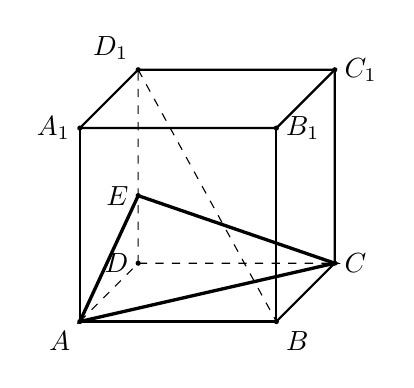
\begin{tikzpicture}[scale=0.78, >=stealth]
  \coordinate (A)  at (0,0);
  \coordinate (B)  at (3.2,0);
  \coordinate (C)  at (4.15,0.95);
  \coordinate (D)  at (0.95,0.95);
  \coordinate (A1) at (0,3.15);
  \coordinate (B1) at (3.2,3.15);
  \coordinate (C1) at (4.15,4.1);
  \coordinate (D1) at (0.95,4.1);
  \coordinate (E)  at (0.95,2.05);

  \draw[thick] (A)--(B)--(B1)--(A1)--cycle;
  \draw[thick] (A1)--(B1)--(C1)--(D1)--cycle;
  \draw[thick] (B)--(C)--(C1);
  \draw[dashed] (A)--(D)--(C) (D)--(D1) (A1)--(D1);
  \draw[dashed] (D1)--(B);
  \draw[very thick] (A)--(E)--(C)--cycle;

  \fill (A)  circle (1.2pt) node[below left] {$A$};
  \fill (B)  circle (1.2pt) node[below right] {$B$};
  \fill (C)  circle (1.2pt) node[right] {$C$};
  \fill (D)  circle (1.2pt) node[left] {$D$};
  \fill (A1) circle (1.2pt) node[left] {$A_1$};
  \fill (B1) circle (1.2pt) node[right] {$B_1$};
  \fill (C1) circle (1.2pt) node[right] {$C_1$};
  \fill (D1) circle (1.2pt) node[above left] {$D_1$};
  \fill (E)  circle (1.2pt) node[left] {$E$};
\end{tikzpicture}
\end{center}
\nopagebreak[4]
\Needspace{4\baselineskip}
\textbf{解析}

\Needspace{5\baselineskip}
建立坐标系

\nopagebreak[4]
\[
A(0,0,0),\quad B(a,0,0),\quad C(a,a,0),\quad D(0,a,0),
\]

设棱柱高为 $h$，$E=(0,a,e)$。平面 $EAC$ 的法向量可取 $\mathbf n=(e,-e,a)$。

\Needspace{5\baselineskip}
由平面夹角为 $45^\circ$，

\nopagebreak[4]
\[
\frac a{\sqrt{2e^2+a^2}}=\frac1{\sqrt2},
\qquad e=\frac a{\sqrt2}.
\]

\Needspace{5\baselineskip}
又 $\overrightarrow{D_1B}=(a,-a,-h)$ 平行于平面 $EAC$，故

\nopagebreak[4]
\[
\mathbf n\cdot\overrightarrow{D_1B}=a^2(2e-h)=0,
\qquad h=\sqrt2a.
\]

\gksubpart{(1)}

\Needspace{5\baselineskip}
由

\nopagebreak[4]
\[
\left|\overrightarrow{AC}\times\overrightarrow{AE}\right|
=a\sqrt{2e^2+a^2}=a^2\sqrt2,
\]

\Needspace{5\baselineskip}
得

\nopagebreak[4]
\[
S_{\triangle EAC}=\frac{a^2}{\sqrt2}.
\]

\gksubpart{(2)}

\Needspace{5\baselineskip}
直线 $A_1B_1$ 与 $AC$ 的公共垂线为竖直方向，端点为 $A_1,A$，所以距离为

\nopagebreak[4]
\[
A_1A=h=\sqrt2a.
\]

\gksubpart{(3)}

\Needspace{5\baselineskip}
平面 $EAC$ 的方程为 $ex-ey+az=0$。点 $B_1=(a,0,h)$ 到该平面的距离为

\nopagebreak[4]
\[
\frac{ea+ah}{\sqrt{2e^2+a^2}}=\frac{3a}{2}.
\]

\Needspace{5\baselineskip}
故三棱锥体积为

\nopagebreak[4]
\[
V=\frac13\cdot\frac{a^2}{\sqrt2}\cdot\frac{3a}{2}
=\frac{a^3}{2\sqrt2}.
\]

\gkanswer{答案（1）：$\dfrac{a^2}{\sqrt2}$}

\gkanswer{答案（2）：$\sqrt2\,a$}

\gkanswer{答案（3）：$\dfrac{a^3}{2\sqrt2}$}

\end{answer}
\begin{answer}
\gksolhead{23}{}

\textbf{题目}：

如图为一台冷轧机的示意图。冷轧机由若干对轧辊组成，带钢从一端输入，经过各对轧辊逐步减薄后输出。

\Needspace{5\baselineskip}
（1） 输入带钢的厚度为 $\alpha$，输出带钢的厚度为 $\beta$，若每对轧辊的减薄率不超过 $r_0$，问冷轧机至少需要安装多少对轧辊？

\nopagebreak[4]
\[
\text{\text{一对轧辊减薄率}}=\frac{\text{\text{输入该对的带钢厚度}}-\text{\text{从该对输出的带钢厚度}}}{\text{\text{输入该对的带钢厚度}}}。
\]

（2） 已知一台冷轧机共有 4 对减薄率为 20\\% 的轧辊，所有轧辊周长均为 1600。若第 $k$ 对轧辊有缺陷，每滚动一周在带钢上压出一个疵点，在冷轧机输出的带钢上，疵点的间距为 $L_k$。为了便于检修，请计算 $L_1$、$L_2$、$L_3$ 并填入下表（轧钢过程中，带钢宽度不变，且不考虑损耗）。

\begin{center}
\begin{tabular}{lrrrr}
\toprule
轧辊序号 & 1 & 2 & 3 & 4 \\
\midrule
疵点间距 $L_k$/mm &  &  &  & 1600 \\
\bottomrule
\end{tabular}
\end{center}
\nopagebreak[4]
\begin{center}% 1999 年全国卷文科第 23 题：冷轧机示意图
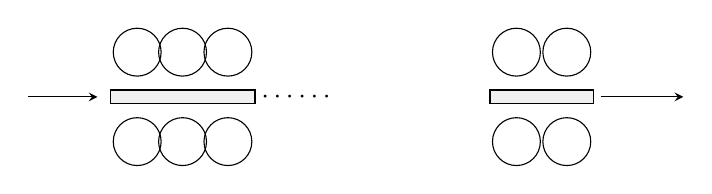
\begin{tikzpicture}[>=stealth, scale=0.8]
  \newcommand{\rollgroup}[1]{%
    \begin{scope}[xshift=#1cm]
      \draw[fill=gray!12] (-1.15,0.0) rectangle (1.15,0.22);
      \foreach \x in {-0.72,0,0.72} {
        \draw (\x,0.82) circle (0.38);
        \draw (\x,-0.60) circle (0.38);
      }
    \end{scope}%
  }
  \draw[->] (-6.15,0.11)--(-5.05,0.11);
  \rollgroup{-3.7}
  \node at (-1.9,0.1) {$\cdots\cdots$};
  \begin{scope}[xshift=2.0cm]
    \draw[fill=gray!12] (-0.82,0.0) rectangle (0.82,0.22);
    \foreach \x in {-0.4,0.4} {
      \draw (\x,0.82) circle (0.38);
      \draw (\x,-0.60) circle (0.38);
    }
  \end{scope}
  \draw[->] (2.95,0.11)--(4.25,0.11);
\end{tikzpicture}
\end{center}
\nopagebreak[4]
\Needspace{4\baselineskip}
\textbf{解析}

\gksubpart{(1)}

\Needspace{5\baselineskip}
每对轧辊最多把厚度乘以 $1-r_0$，经过 $m$ 对轧辊后的厚度满足

\nopagebreak[4]
\[
t_m\ge\alpha(1-r_0)^m.
\]

\Needspace{5\baselineskip}
在 $0<\beta<\alpha$、$0<r_0<1$ 时，要达到 $\beta$ 必须有

\nopagebreak[4]
\[
m\ge\log_{1-r_0}\frac\beta\alpha.
\]

\Needspace{5\baselineskip}
因此至少需要

\nopagebreak[4]
\[
\left\lceil\log_{1-r_0}\frac\beta\alpha\right\rceil
\]

对轧辊。

\gksubpart{(2)}

\Needspace{5\baselineskip}
四对轧辊每次使厚度变为原来的 $0.8$ 倍。第 $k$ 对产生的疵点经过后面各对轧辊后，间距按厚度反比放大，因此

\nopagebreak[4]
\[
L_k=1600\frac{0.8^k}{0.8^4}
=\frac{1600}{0.8^{4-k}}\ \mathrm{mm}.
\]

\Needspace{5\baselineskip}
所以

\nopagebreak[4]
\[
L_1=3125\ \mathrm{mm},\qquad
L_2=2500\ \mathrm{mm},\qquad
L_3=2000\ \mathrm{mm}.
\]

\gkanswer{答案（1）：$\left\lceil\log_{1-r_0}\dfrac{\beta}{\alpha}\right\rceil$ 对轧辊（$0<\beta<\alpha$，$0<r_0<1$）。}

\gkanswer{答案（2）：$L_1=3125\ \mathrm{mm}$，$L_2=2500\ \mathrm{mm}$，$L_3=2000\ \mathrm{mm}$。}

\end{answer}
\begin{answer}
\gksolhead{24}{}

\textbf{题目}：

如图，给出定点 $A(a,0)\ (a>0)$ 和直线 $l:x=-1$。$B$ 是直线 $l$ 上的动点，$\angle BOA$ 的角平分线交 $AB$ 于点 $C$。求点 $C$ 的轨迹方程，并讨论方程表示的曲线类型与 $a$ 值的关系。
\nopagebreak[4]
\begin{center}% 1999 年全国卷文科第 24 题：角平分线轨迹示意图
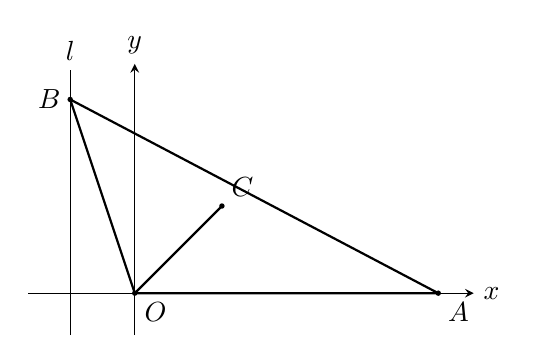
\begin{tikzpicture}[>=stealth, scale=0.82]
  \coordinate (O) at (0,0);
  \coordinate (A) at (4.7,0);
  \coordinate (B) at (-1,3.0);
  \coordinate (C) at (1.35,1.35);

  \draw[->] (-1.65,0)--(5.25,0) node[right] {$x$};
  \draw[->] (0,-0.65)--(0,3.55) node[above] {$y$};
  \draw (-1,-0.65)--(-1,3.45) node[above] {$l$};
  \draw[thick] (B)--(A);
  \draw[thick] (B)--(O)--(A);
  \draw[thick] (O)--(C);

  \fill (O) circle (1.2pt) node[below right] {$O$};
  \fill (A) circle (1.2pt) node[below right] {$A$};
  \fill (B) circle (1.2pt) node[left] {$B$};
  \fill (C) circle (1.2pt) node[above right] {$C$};
\end{tikzpicture}
\end{center}
\nopagebreak[4]
\Needspace{4\baselineskip}
\textbf{解析}

\Needspace{5\baselineskip}
令动点 $B=(-1,u)$，记 $r=\sqrt{1+u^2}=OB$。由角平分线定理

\nopagebreak[4]
\[
\frac{AC}{CB}=\frac{OA}{OB}=\frac ar.
\]

\Needspace{5\baselineskip}
于是

\nopagebreak[4]
\[
x=\frac{a(r-1)}{a+r},\qquad y=\frac{au}{a+r}.
\]

\Needspace{5\baselineskip}
消去参数。由第一式和第二式分别得到

\nopagebreak[4]
\[
r=\frac{a(x+1)}{a-x},\qquad
u=\frac{(a+1)y}{a-x}.
\]

\Needspace{5\baselineskip}
代入 $r^2-u^2=1$，得

\nopagebreak[4]
\[
a^2(x+1)^2-(a+1)^2y^2=(a-x)^2,
\]

\Needspace{5\baselineskip}
即

\nopagebreak[4]
\[
(a-1)x^2+2ax-(a+1)y^2=0.
\]

\Needspace{5\baselineskip}
实际轨迹还满足 $0\le x<a$。当 $a>1$ 时二次项系数异号，表示双曲线；当 $a=1$ 时方程为 $x=y^2$，表示抛物线；当 $0<a<1$ 时可整理为

\nopagebreak[4]
\[
(1-a)x^2+(a+1)y^2=2ax,
\]

表示椭圆。

\gkanswer{答案：轨迹方程为 $(a-1)x^2+2ax-(a+1)y^2=0$；$a>1$ 时为双曲线，$a=1$ 时为抛物线 $x=y^2$，$0<a<1$ 时为椭圆。}

\end{answer}